% !TEX root = ../main.tex

\section{Experimental apparatus}

The EFR is comprised of a series of horizontal and vertical pipes connected with 90 degree elbows as shown in Figure \ref{fig:efr-assembly}. The reactor is essentially a pneumatic conveyor where biomass particles flow through a long pipe with several bends. Dimensions and material information about the EFR apparatus are provided in Figure \ref{fig:efr-geometry}.

\begin{figure}[H]
    \centering
    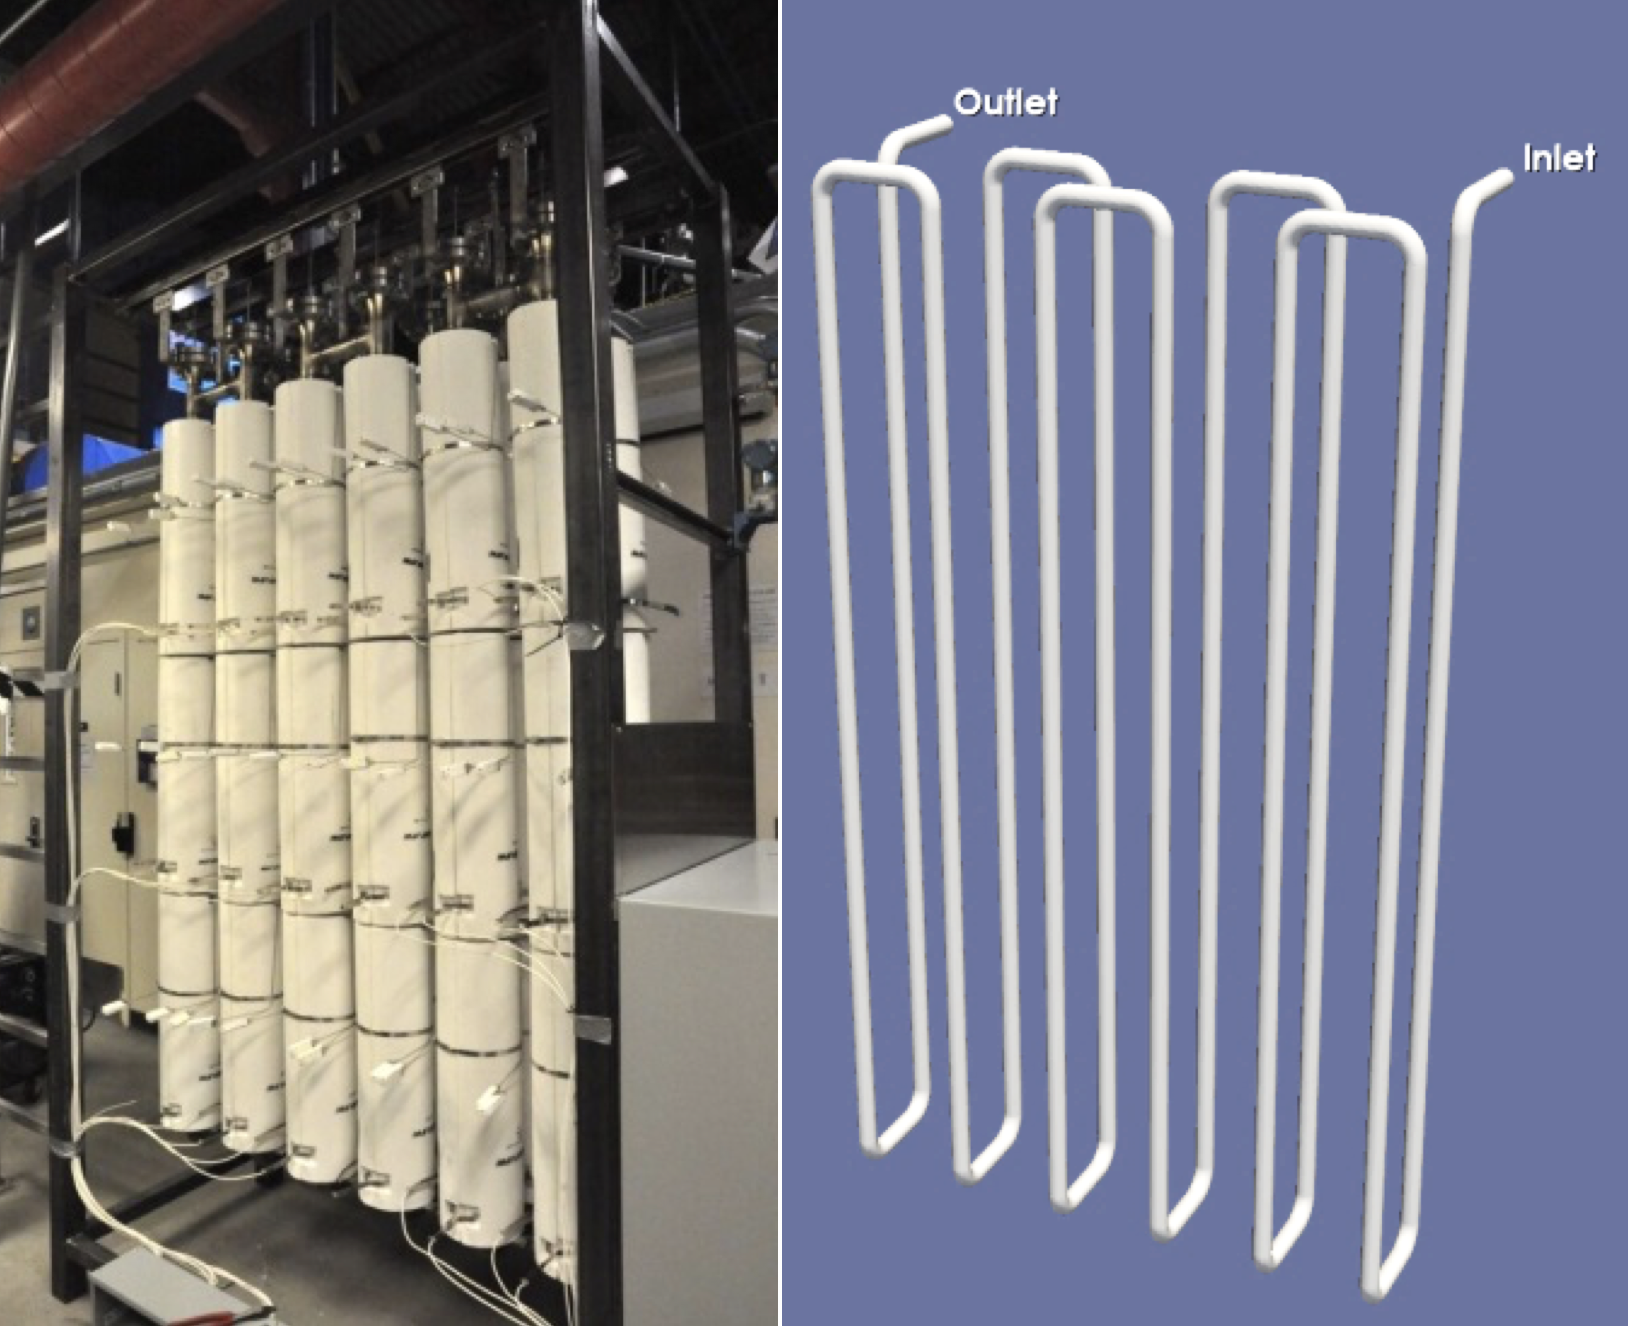
\includegraphics[width=0.8\textwidth]{figures/efr-assembly.png}
    \caption{Left - picture of the EFR assembly with heat jackets, insulation, and thermocouples. Right - CAD representation of the EFR pipe assembly used for MFiX simulations.}
    \label{fig:efr-assembly}
\end{figure}

\begin{figure}[H]
    \centering
    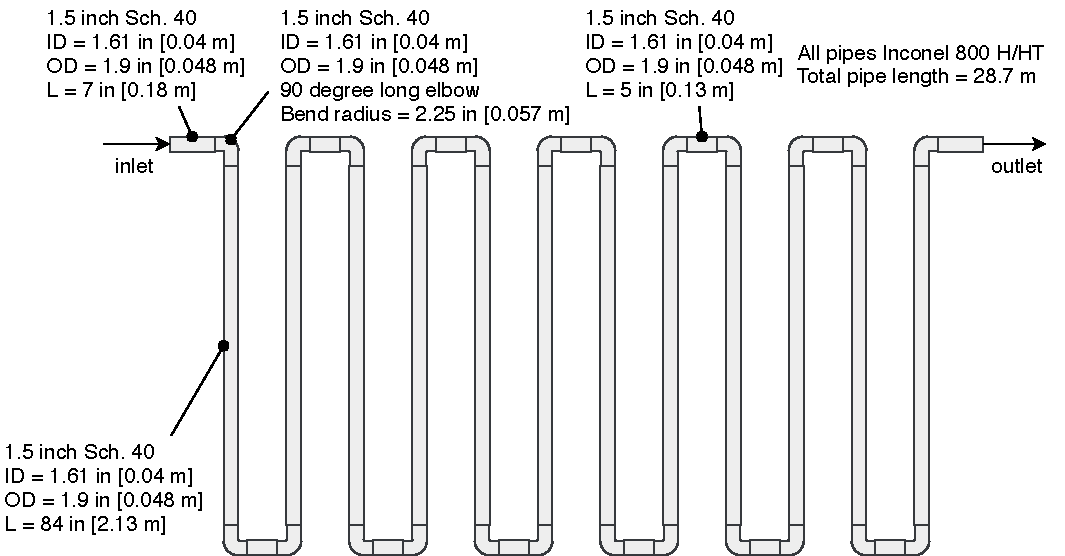
\includegraphics[width=\textwidth]{figures/efr-geometry.pdf}
    \caption{Dimensions and pipe material of the entrained flow reactor. Geometry and material data provided by NREL.}
    \label{fig:efr-geometry}
\end{figure}
